\documentclass{uebblatt}

\begin{document}

\maketitle{9}{}

\begin{aufgabe}{Assoziativität in der Homotopiekategorie}
\emph{Kommt noch.}
\end{aufgabe}

\begin{aufgabe}{Simpliziale Mengen durch Erzeuger und Relationen}
Zeichne für die folgenden Beschreibungen simplizialer Mengen durch Erzeuger und
Relationen das relevante Kolimesdiagramm und gib das Erzeugnis explizit an.
\begin{enumerate}
\item keinerlei Erzeuger
\item genau ein Erzeuger und keine Relationen
\item ein Erzeuger~$v$ in Dimension~1 mit der Relation~$d_0(v) = d_1(v)$
\end{enumerate}
\end{aufgabe}

\begin{aufgabe}{Skelette von simplizialen Mengen}
Sei~$X$ eine simpliziale Menge.

\begin{enumerate}
\item Sei~$x \in X_n$ ein Simplex. Mache dir
klar, dass dieses Datum eine simpliziale Abbildung~$\bar x : \Delta[n] \to \sk_n
X,\ f \mapsto X(f)x$ definiert. Was macht~$\bar x$ anschaulich?
\item Zeige, dass das Bild von~$\SS^{n-1}$ unter der Abbildung
aus~a) schon in~$\sk_{n-1} X$ liegt.
\item Gib die kanonischen Abbildungen des obigen Quadrats an.
Zeige, dass dieses Quadrat ein Pushout-Diagramm ist.
\marginpar{\vspace*{-13em}\hspace*{-6em}$\xymatrixcolsep{1pc}\xymatrixrowsep{1pc}\xymatrix{
  \coprod_{x \in X_{(n)}} \SS^{n-1} \ar[r] \ar[d] &
  \sk_{n-1} X \ar[d] \\
  \coprod_{x \in X_{(n)}} \Delta[n] \ar[r] &
  \sk_n X
}$}
\item Zeige, dass~$X$ ein~$\I$-Zellkomplex ist, wobei~$\I = \{ \SS^{n-1}
\hookrightarrow \Delta[n] \,|\, n \geq 0 \}$.
\end{enumerate}
\end{aufgabe}

\begin{aufgabe}{Beispiele für Kan-Komplexe}
Sei~$\C$ eine kleine Kategorie. Ihr \emph{Nerv} ist die simpliziale Menge~$N\C$
wobei~$(N\C)_m$ die Menge der Diagramme der Form $X_0 \xra{f_0} X_1 \xra{f_1}
\cdots \xra{f_{m-1}} X_m$ in~$\C$ ist.
\begin{enumerate}
\item Zeige, dass~$N\C$ ein innerer Kan-Komplex ist.
\item Zeige, dass~$N\C$ genau dann ein Kan-Komplex ist, wenn~$\C$ ein Gruppoid
ist.
\item Sei~$Y$ ein topologischer Raum. Zeige, dass~$\Sing Y$ ein Kan-Komplex
ist.
\end{enumerate}
\end{aufgabe}

\vfill
\centering
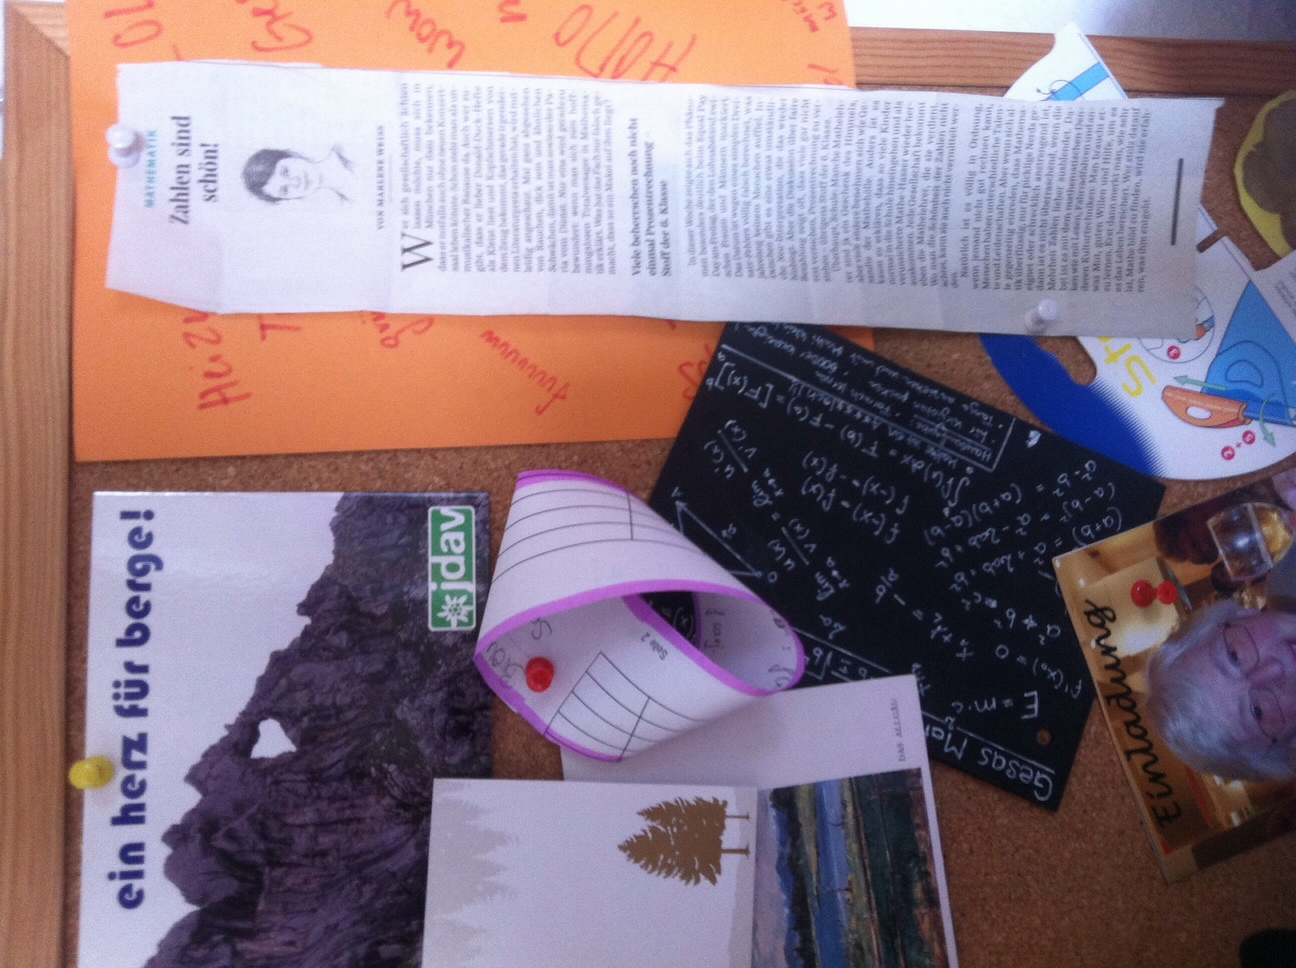
\includegraphics[scale=0.15]{images/moebiuspunkt}
\par

\end{document}

Später vielleicht: BG.
